\documentclass{ctexbook}
\setCJKmainfont{SimSun}[AutoFakeBold,AutoFakeSlant]

%%%%%%%%%%%%% Geometry
\usepackage[a4paper,left=2.5cm,right=2.5cm, bottom=2.5cm,top=2.5cm]{geometry}
\usepackage{amsmath,amssymb,amsthm}
\usepackage{xeCJK} %中日韩文字xeCJK宏包
\usepackage{indentfirst} %设置段首缩进的宏包
\usepackage{cases}%提供了numcases
\usepackage{siunitx}
% \usepackage{extarrows}%提供了\xlongequal 应用
\usepackage{bm}%提供了数学粗体
\usepackage{graphicx}
\usepackage{mathrsfs} %提供了\mathscr
\usepackage{ulem}%提供了\uline{加下划线}而\uwave{加波浪线}则是在文本下面加上波浪线。\sout{中间加横线}
\usepackage{cancel}%提供了划去公式\cancel \bcancel \xcancel \cancelto{新公式}{原公式}
\usepackage{xcolor}
\usepackage{makecell}

\usepackage{listings}
\lstset{
    language=Python,
%     % backgroundcolor=\color{blue!10!gray},%代码块背景色为浅灰色
% %	rulesepcolor= \color{gray}, %代码块边框颜色
% 	breaklines=true,  %代码过长则换行
	numbers=left, %行号在左侧显示
	% numberstyle= \small,%行号字体
% 	commentstyle=\color{gray}, %注释颜色
% 	frame=shadowbox%用方框框住代码块
% 	% frame=single,
% 	escapeinside=``    % 代码包含中文
%     rulesepcolor=\color{red!20!green!20!blue!20},%代码块边框为淡青色
%     %========= 关键字
%     basicstyle = \zihao{-6}\ttfamily,
    numberstyle = \zihao{-6}\ttfamily,
%     commentstyle = \color{green!40!black}\ttfamily,
%     keywordstyle = \color{blue},
%     keywordstyle = [2]\color{teal},
%     stringstyle = \color{magenta},
%     showstringspaces=false,%不显示代码字符串中间的空格标记
%     stringstyle=\ttfamily, % 代码字符串的特殊格式
%     %========= 缩进
%     keepspaces=true, %
%     breakindent=22pt, %
%     tabsize=4, %
%     %========
}
\usepackage{pythonhighlight}

\usepackage[verbose]{hyperref}

\hypersetup{ 
    hidelinks,
    % dvipdfm, % already been used
    pdfstartview=FitH,
    CJKbookmarks=true,
    bookmarksnumbered=true,
    bookmarksopen=true,
    bookmarksopenlevel=0,
    breaklinks=true,
    % colorlinks=true, %注释掉此项则交叉引用为彩色边框(将colorlinks和pdfborder同时注释掉)
    % pdfborder=001,   %注释掉此项则交叉引用为彩色边框
    citecolor=magenta,% magenta洋红 , cyan青色
    linkcolor=blue,
    citecolor=red,
    linkcolor=cyan,
    %linktocpage=true,
    % hyperfootnotes=true, % already been used
    % hyperindex=true, % already been used
}
\usepackage{tikz}
\usetikzlibrary{positioning}
\usetikzlibrary{backgrounds}
\usetikzlibrary{arrows,shapes}
\usetikzlibrary{arrows.meta}
\usetikzlibrary{tikzmark}
\usetikzlibrary{matrix}
\usetikzlibrary{shapes.misc}

\usepackage{pgfplots}

\usepackage[breakable]{tcolorbox}%提供了\colorbox
\tcbuselibrary{skins, breakable, theorems}

\definecolor{tcb_main}{HTML}{5989cf}    % setting main color to be used
\definecolor{tcb_sub}{HTML}{cde4ff}     % setting sub color to be used
\definecolor{tcbproof_main}{rgb}{0.16, 0.28, 0.39}     % setting sub color to be used

\newtcbtheorem{question}{题~(理}
    {enhanced,
     breakable,
     colback = white,
     colframe = cyan,
     colbacktitle = cyan,
     fonttitle = \sffamily\bfseries,
     attach boxed title to top left = {yshift = -2mm, xshift = 5mm},
     boxed title style = {sharp corners},
     separator sign = {).~}
    }{qst}

\newtcbtheorem[number within=chapter]{definition}{定义}
    {fonttitle=\bfseries\upshape,
     fontupper=\slshape,
     colback=red!5!white,
     colframe=red!75!black!70!yellow,
     arc=0mm,
    }{def}
\newtcbtheorem[number within=chapter]{theorem}{定理}
    {fonttitle=\bfseries\upshape,
     fontupper=\slshape,
     colback=blue!5!white,
     colframe=tcb_main,
     arc=0mm,
    }{theo}
\newtcbtheorem[number within=chapter]{corollary}{推论}
    {fonttitle=\bfseries\upshape,
     fontupper=\slshape,
     colback=blue!5!white,
     colframe=tcb_main,
     arc=0mm,
    }{coro}
\newtcbtheorem[number within=chapter]{lemma}{引理}
    {fonttitle=\bfseries\upshape,
     fontupper=\slshape,
     colback=blue!5!white,
     colframe=gray!60!blue,
     arc=0mm,
    }{lemm}
\newtcbtheorem[number within=chapter]{example}{例}% 例题主题样式
    {
    fonttitle=\bfseries\upshape,
    % fontupper=\slshape,
    colback=tcbproof_main!5!white,
    colframe=tcbproof_main,
    % arc=0mm,
    subtitle style={boxrule=0.4pt,
    colback=tcbproof_main!70!gray},
    breakable,
    }{exam}
\newtcolorbox{tcbproof}% 证明主题样式
    {
    sharp corners,
    colback = tcbproof_main!5!white,
    colframe = tcbproof_main,
    boxrule = 0pt,
    leftrule = 5pt % left rule weight
    }
\newtcolorbox{tcbdef}[1]% 样式与定义主题相同,但不作为定义环境
    {
    title=#1,
    fonttitle=\bfseries\upshape,
    fontupper=\slshape,
    colback=red!5!white,
    colframe=red!75!black!70!yellow,
    arc=0mm,
    }
\newtcolorbox{tcbnote}% 注释主题样式
    {
    title=\hbox{\tikz[baseline=-3.8pt]\node[circle,fill=white,inner sep=.2pt]{\color{orange} \textbf{!}}; 注意},
    fonttitle=\bfseries\upshape,
    fontupper=\slshape,
    colback=orange!10!white!95!yellow,
    colframe=orange!89!gray!85!yellow,
    arc=0mm,
    }

% \usepackage{enumerate}
\usepackage{enumitem}%提供了中文编号的enumerate环境
\AddEnumerateCounter{\chinese}{\chinese}{}
\usepackage{wrapfig}

% % Commands for Highlighting text -- non tikz method
\newcommand{\highlight}[2]{\colorbox{#1!17}{$\displaystyle #2$}}
% \newcommand{\highlight}[2]{\colorbox{#1!17}{$#2$}}
% \newcommand{\highlightdark}[2]{\colorbox{#1!47}{$\displaystyle #2$}}

% % Commands for Highlighting text -- non tikz method
\renewcommand{\highlight}[2]{\colorbox{#1!17}{#2}}
% \renewcommand{\highlightdark}[2]{\colorbox{#1!47}{#2}}

\setlength{\parindent}{2\ccwd}  %\parindent表示段首缩进的长度,设置为两个大写字母M的长度

%% 设置罗马数字
\makeatletter
\newcommand{\rmnum}[1]{\romannumeral #1}
\newcommand{\Rmnum}[1]{\expandafter\@slowromancap\romannumeral #1@}
\makeatother
\renewcommand{\Re}{\operatorname{Re}} % Fraktur 体的字母“R”和“I”,改为国标要求使用罗马体的“Re”和“Im”,
\renewcommand{\Im}{\operatorname{Im}}

\begin{document}

\tableofcontents

\chapter{线性代数}

\section{矩阵空间}
    \subsection{Subspace 子空间}
        对于空间$\mathbb{R}^3$,认为:
        \begin{itemize}
            \item 任何过原点的平面是$\mathbb{R}^3$的子空间;
            \item 任何过原点的直线是$\mathbb{R}^3$的子空间;
            \item $\mathbb{R}^3$中的两个子空间的并集不能构成子空间;
            \item $\mathbb{R}^3$中的两个子空间的交集可以构成子空间——零空间。
        \end{itemize}
        
        考虑矩阵$\bm{A}$
        \begin{equation*}
            \bm{A}=\begin{bmatrix}      
                1&1&2\\    
                2&1&3\\    
                3&1&4\\    
                4&1&5
            \end{bmatrix}
        \end{equation*}
        则矩阵$\bm{A}$的列空间是$\mathbb{R}^4$的二维子空间。
        因为$\bm{A}$的列的线性组合表示了$\mathbb{R}^4$中某个过原点的平面。
    \subsection{Colummspace 列空间}
        由线性无关的$n$个$m$维列向量组成矩阵$\bm{A}$,可以把$\bm{A}$看做是由这些向量为基所张成的空间。$\bm{A}\bm{x}$就是把这些向量按特定的权重(列向量$\bm{x}$)组合起来,得到的在这个列空间内的向量。

        这给认识“方程$\bm{A}\bm{x}=\bm{b}$无解”提供了一个新的角度:因为$\bm{b}$不落在$\bm{A}$的列空间中。所以无法找到一个基的组合,使组合与$\bm{b}$重合,但仍可以与$\bm{b}$近似——即组合$\bm{A}\bm{x}$是$\bm{b}$向矩阵$\bm{A}$的列空间做的投影,此时一般认为$\bm{A}\bm{x}$最接近$\bm{b}$。这是就是最小二乘法的本质——投影的目的,实际上是使向量$\bm{b}$到空间$\mathrm{C}(\bm{A})$的欧式距离最短。\footnote[1]{以$\bm{b}\in \mathbb{R}^{3\times 1},A\in \mathbb{R}^{3\times 2}$为例,则表示平面外一点到平面的最短距离是过该点作到平面的垂线段的长度。}

        若设该投影向量为$\bm{p}$,则可知方程$\bm{A}\bm{x}=\bm{p}$有唯一解,$\bm{p}$与$\bm{b}$的误差向量即$\bm{e}=\bm{A}\bm{x}-\bm{b}$。$\bm{e}$垂直于$\mathrm{C}(\bm{A})$,或者说:\textbf{$\bm{e}$位于$\bm{A}$的左零空间}。

        利用向量垂直,可以得到使$\left\Vert \bm{e}\right\Vert_2$最小的近似解,记作$\hat{\bm{x}}$。
        {\color{gray}
        \begin{equation}
            {\bm{p}^\mathrm{T}\bm{e}=0}
        \end{equation}
        {因而得到}
        \begin{equation*}
            {(\bm{A}\hat{\bm{x}})^{\mathrm{T}}(\bm{A}\hat{\bm{x}}-\bm{b})=0}
        \end{equation*}
        发现,用$\bm{p}\perp \bm{e}$会使方程中含有两个$\bm{x}$而不易于求解。}
        注意到$\bm{A}$的每一列都应当与$\bm{e}$垂直,因此有
        \begin{equation}
            \bm{A}^{\mathrm{T}}(\bm{A}\hat{\bm{x}}-\bm{b})=\bm{0}
        \end{equation}
        这里,由于$\bm{A}$列满秩,所以方阵$\bm{A}^{\mathrm{T}}A$满秩、可逆,因此解为
        \begin{equation}
            \hat{\bm{x}}=(\bm{A}^{\mathrm{T}}\bm{A})^{-1}\bm{A}^{\mathrm{T}} \bm{b}
        \end{equation}
        至此,问题似乎已经解决:我们\underline{只需一些矩阵乘法和求逆,即可得出原非齐次超定方程的最小二乘解}。

        但是,还有一些值得研究的问题,例如:是否有一种特定形式的矩阵,可以作为一种变换,把原来的$\bm{b}$向量投影到$\mathrm{C}(\bm{A})$上?
        这个把$\bm{b}$投影为$\bm{p}$的矩阵,和$\bm{A}$的关系表示为:
        \vspace{0.8cm}
        \begin{equation}
            \bm{p}
            =\bm{A}\hat{\bm{x}}
            =\tikzmarknode{ProjMat}{\highlight{red}{$\bm{A}(\bm{A}^{\mathrm{T}}\bm{A})^{-1}\bm{A}^{\mathrm{T}}$}} \bm{b}
        \end{equation}
        \begin{tikzpicture}[overlay,remember picture,>=stealth,nodes={align=left,inner ysep=1pt},<-]
        \path (ProjMat.north) ++ (0,1.5em) node[anchor=south west,color=red!67] (annotation1){\textbf{投影矩阵}$\bm{P}$};
        \draw [color=red!57](ProjMat.north) |- ([xshift=-0.3ex,color=red]annotation1.south east);
        \end{tikzpicture}

        易发现,投影矩阵$\bm{P}$有以下性质:(证明方法直接代入其表达式即可)
        \begin{enumerate}
            \item 是对称方阵。$\bm{P}^{\mathrm{T}}=\bm{P}$
            \item “可折叠”。$\bm{P}^k=\bm{P}\quad(k\in \mathbb{N}^+)$,其直观解释:对于已经在$\mathrm{C}(\bm{A})$上的向量,再次作投影,不发生任何改变。
            \item 降秩。$\bm{P}\in \mathbb{R}^{m\times m}$,但其秩不超过$R(A)=n<m$。
            \item 有固定的特征值0和1。因为:
                \begin{equation}
                    \bm{P}\bm{x}=
                    \left\{\begin{aligned}
                        \bm{x}\;,\quad \bm{x}\in \mathrm{C}(\bm{A})\\
                        0\;,\quad \bm{x}\perp \mathrm{C}(\bm{A})
                    \end{aligned}\right.
                \end{equation}
        \end{enumerate}


    \subsection{Overdetermined Homogeneous Linear System}
        对于过定齐次方程组
        \begin{equation}
            [\bm{A}]_{m\times n}\bm{x}=\bm{0} \quad(m> n)
        \end{equation}
        它倾向于只有唯一零解,因为此时$\bm{A}$通常是非奇异(或列满秩)的。

        我们希望得到一个不平凡解(\emph{non-trivial} solution)$\hat{\bm{x}}$,要求$\hat{\bm{x}}\neq \bm{0}$但使$\bm{A}\bm{x}$几近于$\bm{0}$。

        这个目标可以建模为如下形式:
        \begin{equation}
            \begin{aligned}
                \arg \mathop{\min}_{\bm{x}} \left\Vert \bm{A}\bm{x}\right\Vert_2\\
                \mathrm{s.t.}\; \left\Vert \bm{x}\right\Vert_2=1
            \end{aligned}
        \end{equation}

        这个问题有封闭解:$\hat{\bm{x}}$为$\bm{A}^{\mathrm{T}}\bm{A}$最小特征值对应的特征向量;或者说是$\bm{A}$的最小奇异值对应的奇异向量。

\section{方阵的特征值与特征向量}

        特征值/特征向量的一个重要思想,在于它处理的是这样一种特殊情况——以方阵列为基和以坐标轴(单位阵的列)为基,分别按特征向量加权后组合出的两个向量是平行的——比值为$\lambda$。
        即
        \begin{equation}
            \bm{A}\bm{x}=\lambda \bm{x}
        \end{equation}
        %一旦有上式成立
        特别指出,特征向量不能为零向量。

        给定任意一个方阵,我们希望得出其特征值/特征向量,就需要解上式矩阵方程——但是未知量有两个,已知量只有$\bm{A}$,怎么办呢?

        我们知道,非奇异矩阵的零空间只有零向量。因此把上式整理为关于$\bm{x}$的齐次线性方程组,要使得
        \begin{equation*}
            (\bm{A}-\lambda \bm{I})\bm{x}=\bm{0}
        \end{equation*}
        存在非零解,那么$(\bm{A}-\lambda \bm{I})$只能是奇异矩阵。

        因此
        \begin{equation}
            \left\vert \bm{A}-\lambda \bm{I}\right\vert=0
        \end{equation}
        该式被称为特征方程(\emph{eigenvalue equation})。显然,它是关于$\lambda$的一元$n$次方程。

        好消息是这意味着$n$阶方阵有且仅有$n$个特征值,坏消息是,特征值可能很难求——五次及以上的方程没有根式解。

        \fbox{零空间的求法:对矩阵A进行消元求得主变量和自由变量;给自由变量赋值得到特解;对特解进行线性组合得到零空间。} 


\section{奇异值分解}
        矩阵的奇异值分解(\emph{sigular value decomposition})将是最重要的矩阵分解方式。

        \begin{itemize}
            \item 矩阵是实对称方阵:特征向量正交
            \item 矩阵是共轭对称方阵(\emph{Hermitian Matrix}):特征值为实数,且特征向量正交
            \item 
        \end{itemize}

\chapter{信号处理}

\section{MUSIC算法}
    设有远场区信号源$X_1,X_2\in \mathbb{C}$,其中信号$X_i,\,i=1,2$ 到达 $N_a=3$ 的ULA,由阵元间距$d$和入射角$\theta_i$引起的相位差为$\phi_i$,则
    \begin{equation}
        \phi_i=\frac{2 \pi}{\lambda}d\cos\theta_i=2 \pi f\frac{d\cos\theta_i}{c}
    \end{equation}
    为计算方便,把这个相邻阵元接收信号的相位差用复数表示:
    \begin{equation}
        \varPhi_i=\mathrm{e}^{\mathrm{j}\phi_i}
    \end{equation}
    设$\gamma_i\in \mathbb{C}$表示信源$i$传播到ULA的参考阵元(通常就取第一个阵元)的过程中引起的幅值和相位的变化,设阵元$j$处收到的信号为$Y_j$,则
    \begin{equation}
        Y_j=\gamma_1 X_1 \varPhi_1^{(j-1)} + \gamma_2 X_2 \varPhi_2^{(j-1)} \quad j=1,\cdots,N_a=3
    \end{equation}
    注意,$Y_j$和$X_i$本身都是时域信号的采样点,因此是向量的形式。

    写成矩阵形式:
    \begin{equation}\label{Equ: rx of ULA}
         \tikzmarknode{Y}{\highlight{red}{$\displaystyle \begin{bmatrix}Y_1\\Y_2\\Y_3\end{bmatrix}$}}
         =\tikzmarknode{X}{\highlight{blue}{$\begin{bmatrix}1 &1\\\varPhi_1 &\varPhi_2\\\varPhi_1^2 &\varPhi_2^2\\\end{bmatrix}$}}
         \begin{bmatrix}
            \gamma_1 X_1\\
            \gamma_2 X_2
        \end{bmatrix}
    \end{equation}
    \begin{tikzpicture}[overlay,remember picture,>=stealth,nodes={align=left,inner ysep=1pt},<-]
    \path (Y.south) ++ (0,-1em) node[anchor=north east,color=red!67] (annotation1){$\bm{Y}$\textbf{矩阵}};
    \draw [color=red!57](Y.south) |- ([xshift=-0.3ex,color=red]annotation1.south west);
    \path (X.south) ++(0,-1em) node[anchor=north west,color=blue!67] (annotation2){$\bm{\varPhi}$\textbf{矩阵}};
    \draw [color=blue!57](X.south) |- ([xshift=-0.3ex,color=blue]annotation2.south east);
    \end{tikzpicture}
    \vspace{1cm}

    在实际问题中,往往已知$\bm{Y}$,而信源和传播路径未知,要由此直接解出$\bm{\varPhi}$似乎不可能。

    回想一下学过的数学知识,在满足什么样的条件时,我们可以仅通过一个已知量$b$,就确定方程
    \begin{equation*}
        k_1 x_1 + k_2 x_2 = b
    \end{equation*}
    的参数$k$呢?

    在线性代数里,如果两个向量线性无关,那么这两个向量按任意不全为零的系数$k_1,k_2$加权求和都不可能得到零向量。

    因此,如果这里$b$是零向量,而$x_1,x_2$满足线性无关时,就只有$k_1=k_2=0$能满足原方程。换言之,在涉及线性无关向量组的运算中,如果把方程整理(或寻找一种变换)使等式右边为0,左边为线性无关向量做 linear combanation 的形式,那么就必然得出加权系数为0的结论。

    受以上启发,我们对问题增加新的限制条件:\textbf{各个信源信号彼此是线性无关的}。则此处$\gamma X_1$和$\gamma X_2$线性无关。对\hyperref[Equ: rx of ULA]{式(\ref*{Equ: rx of ULA})}两边左乘加权系数向量$\bm{C}\in \mathbb{C}^{N_a}$:
    \begin{equation}
            c_1Y_1+c_2Y_2+c_3Y_3
        =
        \begin{bmatrix}
            c_1 &c_2 &c_3
        \end{bmatrix}
        \begin{bmatrix}1 &1\\\varPhi_1 &\varPhi_2\\\varPhi_1^2 &\varPhi_2^2\\\end{bmatrix}
        \begin{bmatrix}
            \gamma_1 X_1\\
            \gamma_2 X_2
        \end{bmatrix}
    \end{equation}

    我们需要找到合适的$\bm{C}\neq 0$,使$\bm{C}\bm{Y}=0$。如果这样的$\bm{C}$存在,那么加权系数向量$\bm{C}\bm{\varPhi}$就是零向量,进而求出$\bm{\varPhi}$。

    那么这样的$\bm{C}$存不存在呢?事实上,由于天线数量$N_a$大于信源数量,即$\bm{\varPhi}$的行数大于列数,因此矩阵$\bm{Y}=\bm{\varPhi}\bm{X}$的秩一定不大于$\bm{\varPhi}$的列数。即$\mathrm{R}(Y)\leqslant \min\{\mathrm{R}(\bm{\varPhi}),\mathrm{R}(\bm{X})\}\leqslant 2$。\footnote[1]{$\bm{\varPhi}$可以看作是范德蒙矩阵的一部分,此处只要$\theta_1\neq\theta_2$则$\bm{\varPhi}$ 就是列满秩的;而由于线性无关所以 $\bm{X}$行满秩,因此它们乘积的秩一般而言为2,即信源个数。}  因此矩阵$\bm{Y}$行降秩,所以$Y_1,Y_2,Y_3$必然是线性相关的,存在不全为零的系数$c_1,c_2,c_3$,使
    \begin{equation*}
        c_1Y_1+c_2Y_2+c_3Y_3=0
    \end{equation*}

    对于有$N_s$个采样点的接收信号组成的矩阵$\bm{Y}_{N_s\times 3}$,如何求解$\bm{C}\bm{Y}=0$?显然,该方程
    \begin{equation}
        \begin{bmatrix}
            Y_1[1] &Y_2[1] &Y_3[1]\\
            Y_1[2] &Y_2[2] &Y_3[2]\\
            \vdots &\vdots &\vdots\\
            Y_1[N_s] &Y_2[N_s] &Y_3[N_s]
        \end{bmatrix}
        \begin{bmatrix}
            c_1\\ c_2\\ c_3
        \end{bmatrix}
        =
        \begin{bmatrix}
            0\\
            0\\
            \vdots \\
            0
        \end{bmatrix}
    \end{equation}
    是关于$\bm{C}$的超定(\emph{overdetermined})方程组,而且还是齐次(\emph{homogenous})的。

    超定方程组通常无解,我们只能得到近似解,并选取一个量化误差的指标使近似解最优。最常的指标是平方和(或者欧氏距离),这种求近似解的方法就是\textbf{最小二乘法}。


    % 对于
    % \begin{equation}
    %     \begin{bmatrix}
    %         y_1(1) &y_1(2) &\cdots &y_1(N)\\
    %         y_2(1) &y_2(2) &\cdots &y_2(N)\\
    %         y_3(1) &y_3(2) &\cdots &y_3(N)
    %     \end{bmatrix}
    %     =
    % \end{equation}\left\lfloor  \right\rceil 
\section{统计信号处理的估计理论}
    本章节介绍从含有随机性的时间序列(以下简称随机信号)中提取未知参数的问题。
    \subsection{参数估计的数学模型}
        几乎任何来自物理世界的的数据都具有随机性,一组时间序列可以看作是参数服从特定分布的随机过程$\bm{\mathrm{x}}$的一个实现,记作$\bm{x}$。为了简化问题,通常认为随机过程$\bm{\mathrm{x}}$是\emph{各态历经}(Ergodic)的,即随机过程中的任何一个样本函数$\bm{x}$都含有随机过程的全部统计信息。

        通常问题为:需要通过观测到的随机信号$\bm{x}$来估计$\mathrm{\bm{x}}$的某个或某些参数,参数用向量$\bm{\theta}$表示。

        为了得到更优的估计,我们应确定一个合适的\emph{估计量}(Estimator),记作$\hat{\bm{\theta}}$,它是关于样本数据的函数,并应当充分利用样本的信息。

        至此,问题描述为:随机信号$\bm{x}$服从参数为$\bm{\theta}$的某分布,已知$\bm{x}$的样本$[x(0),\,x(1),$ $\,\cdots,\,x(N-1);\bm{\theta}]$,求尽可能\footnote[2]{我们希望估计量越接近真值越好,但怎样评估估计量的性能,以得到最适合当前问题的估计量,这个问题将在下一节讨论。}接近真值$\bm{\theta}$的估计量$\hat{\bm{\theta}}$。

        求解参数估计问题的两个关键:
        \begin{enumerate}
            \item 对随机信号$\bm{x}$建模。对$\bm{x}$的分布类型提出一个合理的假设,即得出$\bm{x}$服从的PDF。模型的选取要求其既方便数学推导出闭合形式的估计量,又贴合实际问题。
            \item 确定最佳/准最佳估计量。估计量$\hat{\bm{\theta}}$通常是关于样本数据和其他已知参数的函数,它应当按你所希望的方式接近其真值$\bm{\theta}$。
        \end{enumerate}

        对于第一个问题,通常有两种方式得出随机信号的PDF。

        经典方法是认为参数$\bm{\theta}$是一组确定的未知数。
        与之相对的是\emph{贝叶斯(Bayesian)估计},认为参数本身是服从某种分布(需要依据先验知识假定,例如均匀分布)的随机变量,因此它具有先验PDF。
        这里用两个例子说明之。

        \begin{example}{服从正态分布的单随机变量均值估计概率模型}{服从正态分布的单变量均值估计概率模型}
            对于长度为1的随机信号$\bm{x}=x(0)$,其值服从方差为$\sigma^2$的正态分布,现需要估计其均值。求随机信号$\bm{x}$的PDF。
            \tcbsubtitle{解:}
            \setlength{\parindent}{2\ccwd}
            在经典方法中,认为分布的参数是未知的确定量,因此这里无论是估计均值还是估计方差,或者两者,都不影响PDF的形式——把所有参数当做已知量即可。PDF为
            \begin{equation}
                p(\bm{x};\bm{\theta})=p(x(0);\theta)=\frac{1}{\sqrt{2 \pi\sigma^2}}\mathrm{exp}\left[-\frac{(x(0)-\theta)^2}{2 \sigma^2}\right]
            \end{equation}
            须指出,$p(\bm{x};\bm{\theta})$的分号表示该PDF是依赖于给定向量$\bm{\theta}$的一族PDF曲线。而$p(\bm{x},\bm{\theta})$中的逗号表示这是一个联合概率密度函数,联合的随机变量用逗号分隔。
        \end{example}

        \begin{example}{服从正态分布的多变量均值估计概率模型}{服从正态分布的多变量均值估计概率模型}
            现收集有某地连续$N$天的道琼斯(\emph{Dow-Jones})工业平均指数的数据$x(0),\,x(1),\,\cdots,\,x(N-1)$,数据整体随时间呈上升趋势,但细节仍有较大起伏。求该地区道琼斯工业平均指数服从的PDF。
            \tcbsubtitle{解:}
            \setlength{\parindent}{2\ccwd}
            我们用直线和高斯白噪声(White Gaussian Noise, WGN)拟合数据,设
            \begin{equation}\label{Equ: 含有加性白噪声的随机信号}
                x(n)=\theta_1+\theta_2n+w(n) \;\quad n=0,1,\cdots,N-1
            \end{equation}
            从经典估计的角度来看,直线$\theta_1+\theta_2n$是时域一条确定的直线,每个数据点都是在这条定直线的基础上加一个零均值、方差为$\sigma^2$的随机数得到,换言之,每个样本点中随机的成分是正态随机变量$w(n)$的实现。而从贝叶斯估计的角度,由于参数是随机变量,每次对随机信号的观测都对应一条不同的直线,每一个样本点应当视作是$\theta_1,\theta_2,w(n)$的共同实现。

            须指出,模型如\hyperref[Equ: 含有加性白噪声的随机信号]{式(\ref*{Equ: 含有加性白噪声的随机信号})}不依赖于估计方法,这是为了贴合实际问题作出的人为假设。不同估计方法造成的差异体现在PDF的推导上。

            对于这种含有加性白噪声的数字信号模型,通常%\footnote[2]{认为时域的每一次采样都是独立的?}把
            随机信号看作一组联合的随机变量。
            
            因此经典估计认为$\bm{x}$服从的PDF为
            \begin{equation}
                p(\bm{x};\bm{\theta})=\frac{1}{(2\pi\sigma^2)^{\frac{N}{2}}}\mathrm{exp}\left[-\frac{1}{2\sigma^2}\sum_{n=0}^{N-1}(x(n)-\theta_1-\theta_2n)^2\right]
            \end{equation}
            
            而贝叶斯估计认为$\bm{x}$服从的PDF为
            \begin{equation}
                p(\bm{x},\bm{\theta})=p(\bm{x}|\bm{\theta})p(\bm{\theta})
            \end{equation}
            其中$p(\bm{\theta})$是先验PDF,表示在数据观测以前关于$\bm{\theta}$的先验知识;$p(\bm{x}|\bm{\theta})$是条件PDF,表示在给定$\bm{\theta}$的前提下由数据$\bm{x}$提供的知识。
        \end{example}

    \subsection{估计量的性能}
        已经指出,估计量是样本值的函数:
        \begin{equation*}
            \hat{\bm{\theta}}=g(\bm{x})
        \end{equation*}
        因此估计量是一个随机变量,它的性能由其PDF完全描述,并且也只能从统计的角度描述。

        通常从以下几个方面考察估计量的性能:
        \begin{enumerate}

            \item 从估计量与样本数量$n$的关系考虑;
                
                估计量的PDF随观测次数的变化的性质需引起重视,因为\uline{这决定了我们增加试验次数是否真的能使估计的结果更准确}——如果是,那么可以适当增加观测数;否则只是在浪费时间。
                
                我们用随机变量序列$\hat{\theta}_n$来表示估计量对观测数$n$的依赖关系。例如其中$\hat{\theta}_i$表示用$n=i$个样本来估计真值$\theta$的一个估计量。
                \begin{definition}{一致估计量}{一致估计量}
                    给定$n$个观测$\bm{x}_1,\,\bm{x}_2,\,\cdots,\,\bm{x}_n$,估计量$\hat{\theta}_n$是这$n$个观测的函数。若对于真值的所有可能取值$\theta$,$\hat{\theta}_n$都满足依概率收敛于真值,则称该估计量为一致(consistent)估计量(或称为相合估计量)。即
                    \begin{equation}
                        \lim_{n \to \infty}{\mathrm{Pr}\left\{|\hat{\theta}_n-\theta|\geqslant\epsilon\right\}=0}
                    \end{equation}
                    其中$\epsilon$为任意小的正数。
                    % 该式表示\emph{估计量$\hat{\theta}$依概率收敛于真值$\theta$}。
                    \tcblower
                    “$\hat{\theta}_n$依概率收敛于$\theta$”有时也记作:
                    \begin{equation}
                        \mathrm{p}\lim_{n \to \infty}\left(\hat{\theta}_n\right)=\theta
                    \end{equation}
                \end{definition}
                在思考这个概念时,应当把估计量的PDF看做是依赖于$n$的一族曲线,而\emph{一致性(consistency)}则是描述了这一族曲线随着$n\rightarrow\infty$逐渐压缩成一个冲激函数(即收敛于一个具体的数值$\theta$)或者逐渐形成某个特殊分布的形状\footnote[2]{TODO:这是贝叶斯学派的观点,是这样吗?}(即收敛于一个已知参数的随机变量$\theta$)。


            \item 从估计量的期望考虑;
                \begin{definition}{无偏估计量}{无偏估计量}
                    若对于真值的所有可能取值$\theta$以及任意有限的观测次数$n$,估计量$\hat{\theta}_n$的期望\footnotemark[1]都与之相等,则称该估计量为无偏(Unbiased)估计量。即
                    \begin{equation}
                        E\left[\hat{\theta}_n\right]=\theta \;,\quad n=1,2,\cdots
                    \end{equation}
                    \tcblower
                    反之,不满足以上条件的估计量为有偏(Biased)估计量,称其期望与真值的差值为\emph{偏差}(或称偏误),写作
                    \begin{equation}
                        \mathrm{b}(\hat{\theta}_n)=E\left[\hat{\theta}_n\right]-\theta
                    \end{equation}
                \end{definition}
                
                % 无偏是一个很好的性质,但有时为了减小估计量的方差而采用有偏估计量。
                \footnotetext[1]{TODO:又一说为已知$\theta$的条件期望?}


            \item 综合以上1、2考虑:
                \begin{definition}{渐进无偏估计量}{渐进无偏估计量}
                    给定$n$个观测$\bm{x}_1,\,\bm{x}_2,\,\cdots,\,\bm{x}_n$,估计量$\hat{\theta}_n$是这$n$个观测的函数。若对于真值的所有可能取值$\theta$,估计量的期望在$n\rightarrow\infty$时收敛于真值,则称该估计量为渐进无偏(asymptotic unbiased)估计量。即
                    \begin{equation}
                        \lim_{n \to \infty}{E\left[\hat{\theta}_n\right]]}=\theta
                    \end{equation}
                \end{definition}
                
                \begin{tcbnote}
                    无偏、一致、渐进无偏三者的区别和联系。
                    \begin{itemize}
                        \item 估计量的无偏性与样本个数$n$无关,它是一个有限样本特性,也称小样本特性。
                        \item 估计量的渐进无偏性需要在$n\rightarrow\infty$时根据$\mathrm{E}\left[\hat{\theta}\right]$的极限值判断,与一致性一同被称为无限样本特性(或大样本特性)。
                        \item 若估计量的期望等于真值(无偏性),则其极限必然也为真值(渐进无偏性)。
                        \item “依概率收敛”是一个相对宽松的条件。估计量依概率收敛于真值(一致性),并不能得出估计量的期望在$n\rightarrow\infty$的极限等于真值(渐进无偏性)!(可以举一个让期望趋于无穷的反例,见《概率导论》P298例5.7)
                        \item 若估计量的方差满足在$n\rightarrow\infty$的极限为0,且估计量是渐进无偏的,则估计量具有一致性。这是因为“依均方收敛”的条件强于“依概率收敛”。
                
                    \end{itemize}


                    \begin{center}
                    \begin{tikzpicture}
                        \matrix (m)[row sep=6em,column sep=0.5cm,minimum width=1em]
                        {
                            \node [label=above:{\color{gray} 无偏性}] (无偏性){$E\left[\hat{\theta}_n\right]=\theta$};& &\node [label=above:{\color{gray} 渐进无偏性}] (渐进无偏性) {$\lim\limits_{n \to \infty}{E\left[\hat{\theta}_n\right]=\theta}$};\\
                            &\node [label=below:{\color{gray} 一致性}] (一致性){$\mathrm{p}\lim\limits_{n \to \infty}\left(\hat{\theta}_n\right)=\theta$}; &  \\
                        };
                    \path[-stealth]
                        (无偏性) edge [double] node [left] {} (渐进无偏性)
                        (渐进无偏性) edge [double] node [above,sloped] {\fontsize{6}{7} $\displaystyle \lim_{n \to \infty}{\mathrm{Var}\left[\hat{\theta}_n\right]=0}$} (一致性)
                        % (一致性) edge [dashed] node [right] {} (渐进无偏性)
                    ;
                    \end{tikzpicture}
                    \end{center}
                \end{tcbnote}

            \item 从估计量的方差考虑:
            
                估计量的方差越小,说明估计结果越稳定;但估计量仍可能是有偏的、也可能不以概率收敛。


            \item 从估计量到真值的均方误差考虑:
                \begin{definition}{估计量的均方误差}{估计量的均方误差}
                    估计量$\hat{\theta}$到真值$\theta$的均方误差(Mean Square Error, MSE),记作$\mathrm{mse}\left(\hat{\theta}\right)$,定义为随机变量$(\hat{\theta}-\theta)^2$的期望。即
                    \begin{equation}
                        \mathrm{mse}\left(\hat{\theta}\right)=E\left[(\hat{\theta}-\theta)^2\right]
                    \end{equation}
                \end{definition}

                均方误差同时考虑到了估计量的偏差和方差所带来的误差。因此能更全面地体现估计量的性能。

        \end{enumerate}

    % \subsection{MVU Estimator 最小方差无偏估计}
    \subsection{估计量的最小均方误差准则}

        目的:找到用来估计\emph{未知确定性参数}的最佳估计量。

        如何定义“最佳”?我们需要给出一个量化的准则,这里使用的就是\uline{最小均方误差}准则。使估计量到真值的MSE最小的估计量,可以称为最小均方误差(Minimum MSE)估计量,但为什么研究的却是最小方差无偏(Minimum Variance Unbiased, MVU)估计量呢?

        这是因为最小均方误差(MMSE)估计量通常是不可实现的:
        \begin{equation}
            \begin{aligned}
                \mathrm{mse}\left(\hat{\theta}\right)
                &=E\left\{\left[\left(\hat{\theta}-E(\hat{\theta})\right)+\left(E(\hat{\theta})-\theta\right)\right]^2\right\}\\
                &=E\left\{\left(\hat{\theta}-E(\hat{\theta})\right)^2\right\}+2E\left\{\hat{\theta}-E(\hat{\theta})\right\}\cdot \mathrm{b}\left(\hat{\theta}\right)+\mathrm{b}^2\left(\hat{\theta}\right)\\
                &=\mathrm{Var}\left(\hat{\theta}\right)+\mathrm{b}^2\left(\hat{\theta}\right)
            \end{aligned}
        \end{equation}
        这是一个很重要的公式。它说明估计量到真值的MSE是估计量的方差和偏差引起的。在很多统计问题中都存在等式右边两项的权衡——方差的减少总是伴随着偏差的增大。

        但也可以看到,MMSE准则因为引入真值参与运算而使之成为一般不可实现的估计量\footnote[1]{在几种极端情况下是可实现的。见《统计信号处理》P17},它不能写成只关于样本数据的函数——估计量的偏差还是关于真值的函数。

        为了避免不可实现的估计量,我们约束偏差为零,即在无偏估计的前提下使估计量的方差最小,得到最小方差无偏(MVU)估计量。

        MVU估计量 的MSE就是它的方差,而方差作为一个统计量可以由样本数据得出\footnote[1]{样本方差是方差的无偏估计量。},因此MUV估计量是可实现的估计量,下面讨论其存在性。

        \subsubsection{MVU估计量的存在性}

            MVU估计量要存在,首先应满足无偏估计量的存在性,然后在所有的无偏估计量中,若对所有可能的真值取值$\theta$,都存在某个无偏估计量的方差始终比其他无偏估计量的方差小,则这个估计量就是MVU估计量。

            你可能会问:估计量的方差为什么会随真值$\theta$取值变化而变化?前面已经提到,观测次数$n$可能会影响估计量的PDF曲线,这是因为估计量的构造和样本数目有关。而事实上参数真值影响了样本的分布,因此估计量的PDF也会随之变化。

        \subsubsection{MVU估计量的求法}
            目前没有一种总是能得到MVU估计量的“转动摇把”(turn-the-crank)的方法。后面的章节将详细讨论如何在已知存在性时,求出MUV估计量,这里只作为一个引子简单介绍。
            
            
            \begin{enumerate}[label=法\chinese*:,itemjoin=\\\hspace*{\parindent}, leftmargin=1.4cm, rightmargin=2.5cm]
            % \renewcommand*\labelenumi{法\zhnum{\theenumi}}
            % \AddEnumerateCounter{\chinese}{\chinese}{}
                \item 确定 Cramer-Rao 下限(Cramer-Rao lower bound, CRLB),然后检查估计量是否满足Cramer-Rao下限。
                \item 应用 Rao-Blackwell-Lehmann-Scheffe(RBLS)定理。
                \item 进一步限制无偏估计量是线性的,然后找到线性无偏约束下的最小方差估计。
            \end{enumerate}

    \subsection{Cramer-Rao 下限}
        我们希望对任何无偏估计量,都能确定其方差的下限。在最理想的情况下,对于未知参数的所有取值,如果某个无偏估计量的方差都达到了此下限,那么它就是MVU估计量。在最恶劣的情况下,即使不存在 MVU估计量 ,它也能为比较无偏估计量的性能提供一个标准。

        Cramer-Rao下限 (CRLB),由 Harald Cramer 和 Calyampudi Radhakrishna Rao 得名。事实上,历史上的研究者提出了很多种估计量的方差下限,但是 CRLB 是最容易确定的。
        
        CRLB 给出了一个确定性参数的无偏估计量的方差下限。它的最简单形式是:任何无偏估计的方差都不小于 Fisher 信息的倒数。一个达到了方差下限的无偏估计被称为完全高效的(fully efficient)。

        给定估计量偏差,CRLB 还可以用于确定有偏估计的界限。在一些情况下,有偏估计的MSE可能小于无偏估计的 CRLB。


        \subsubsection{关于参数估计的精度的考虑}
        前面已经提到,对于某个具体的估计量,它的PDF越集中于真值附近(对于一般估计量来说就是MSE越小,对无偏估计量来说就是方差越小),则估计精度越高。这说的是不同估计量的性能问题,但实际上除了估计量的选取影响了估计精度外,问题的概率模型自身——或者说随机信号的PDF,才是限制估计精度的首要原因。

        例如,如果数据服从的PDF对未知参数的依赖性较弱,或者考虑最极端的情况:PDF根本与未知参数无关,那么我们不可能以任何精度来估计参数。一般而言,PDF受未知参数的影响越大,所得估计越好。下面的例子说明了这一点。

        \begin{example}{比较从不同功率的WGN中估计DC电平的精度}{比较从不同功率的WGN中估计DC电平的精度}
            设有WGN $w(n)\sim\mathcal{N}(0,\sigma^2)$。随机信号建模为一个未知但确定的DC量$A$与WGN的叠加。现每次观测单个样本:
            \begin{equation*}
                x(0)=A+w(0)
            \end{equation*}
            提出$A$的一个无偏估计量$\hat{A}$,比较当$\sigma^2$分别取值$\sigma_1^2$和$\sigma_2^2$时($\sigma_1^2<\sigma_2^2$),估计量$\hat{A}$的精度。如何量化这种“精度”?
            \tcbsubtitle{解:}
            \setlength{\parindent}{2\ccwd}
            \begin{equation*}
                 E\left[x(0)\right]=A+E\left[w(0)\right]=A
            \end{equation*}
            因此$\hat{A}=x(0)$是无偏估计量。
            
            为了比较随机信号PDF对$\hat{A}$的估计精度的影响,先写出PDF:
            \begin{equation*}
                p_i(x(0);A)=\frac{1}{\sqrt{2\pi\sigma_i^2}}\mathrm{exp}\left[-\frac{1}{2\sigma_i^2}\left(x(0)-A\right)^2\right] \quad i=1,2
            \end{equation*}
            该式既是估计量$\hat{A}$的PDF,也是随机信号的PDF,它们都依赖于真值$A$。
            
            从该式看出,当$\sigma^2$取值越大,$A$对PDF的影响越不明显。极端情况当$\sigma\rightarrow\infty$时,PDF几乎与$A$无关。

            下面引入\emph{似然函数}的概念,以便于定量说明该问题。
            如果$x(0)$给出,把PDF看作是关于$A$的函数,就得到了{似然函数},如下图\hyperref[Fig: 不同噪声功率下未知参数的似然函数]{图\ref*{Fig: 不同噪声功率下未知参数的似然函数}}所示。


            \begin{center}
                \begin{tikzpicture}[baseline, scale=0.7]
                    \begin{axis}[
                    width=8cm,
                    axis lines=left,
                    % scaled ticks=false,
                    yticklabel pos=upper,
                    ymin=0,ymax=1.4,
                    xmin=-0.5,xmax=6.5,
                    xticklabel style={
                    rotate=45,
                    anchor=north east,
                    },
                    xtick={(\MU-3*\SIGMA),\MU,(\MU+3*\SIGMA)},
                    xticklabels={$x(0)-3\sigma_1$,$x(0)$,$x(0)+3\sigma_1$},
                    axis y line=middle,
                    % xlabel={$\hat{A}$},
                    ]
                    % density of Normal distribution:
                    \newcommand\MU{3}
                    \newcommand\SIGMA{(1/3)}
                    % \addplot [red,domain=\MU-3*\SIGMA:\MU+3*\SIGMA,samples=201]
                    \addplot [orange,domain=0:6,samples=201]
                    {exp(-(x-\MU)^2 / 2 / \SIGMA^2)/ (\SIGMA * sqrt(2*pi))};
                    \legend{$\sigma_1^2=\frac 19$}
                    \end{axis}
                    \node at (7cm,0) {\scriptsize $A$};
                    \node at (1.8,5.4) {\scriptsize $p_1(x(0);A)$};
                \end{tikzpicture}
                \hspace*{20pt}
                \begin{tikzpicture}[baseline, scale=0.7]
                    \begin{axis}[
                    width=8cm,
                    axis lines=left,
                    yticklabel pos=upper,
                    ymin=0,ymax=1.4,
                    xmin=-0.5,xmax=6.5,
                    xticklabel style={
                    rotate=45,
                    anchor=north east,
                    },
                    xtick={(\MU-3*\SIGMA),\MU,(\MU+3*\SIGMA)},
                    xticklabels={$x(0)-3\sigma_2$,$x(0)$,$x(0)+3\sigma_2$},
                    axis y line=middle,
                    % xlabel={$\hat{A}$},
                    ]
                    % density of Normal distribution:
                    \newcommand\MU{3}
                    \newcommand\SIGMA{1}
                    \addplot [red,domain=\MU-3*\SIGMA:\MU+3*\SIGMA,samples=201]
                    {exp(-(x-\MU)^2 / 2 / \SIGMA^2) / (\SIGMA * sqrt(2*pi))};
                    \legend{$\sigma_2^2=1$}
                    \end{axis}
                    \node at (7cm,0) {\scriptsize $A$};
                    \node at (1.8,5.4) {\scriptsize $p_2(x(0);A)$};
                \end{tikzpicture}                
            \end{center}

            \begin{wrapfigure}[1]{r}{\textwidth}
                \vspace{-20pt}
                \caption{\kaishu 不同噪声功率下未知参数的似然函数}\label{Fig: 不同噪声功率下未知参数的似然函数}
            \end{wrapfigure}
            ~\\

            直观地看,似然函数的“尖锐程度”体现了我们估计未知参数的精度。而“尖锐程度”可由函数的曲率刻画。因此提出用函数曲率来表示估计精度。

            考察\emph{对数似然函数}的曲率——即似然函数的{\color{red!80!black} 对数}的二阶{\color{red!80!black} 负}导数:
            \begin{equation}
                -\frac{\partial^2\ln p(x(0);A)}{\partial A^2}=-\frac{\partial }{\partial A}\left[\frac{1}{\sigma^2}\left(x(0)-A\right)\right]=\frac{1}{\sigma^2}
            \end{equation}
            该式说明正态分布曲线在极值点处的曲率等于方差的倒数。因此方差越大,曲率越小,曲线越平缓,估计的精度越差。

            在这个例子中,曲率只和方差有关,与观测值无关,这只是因为在PDF中两者是分离的,但一般来说对数似然函数的曲率也是关于样本$x(n)$的函数——也就是说,似然函数是样本的随机变量函数,并且依赖于未知参数,所以它的对数的曲率也一般是关于样本和参数的函数。

            因此我们先对$p(x(0);A)$取期望,使它仅为$A$的函数。得到 对数似然函数曲率 更一般的度量:
            \begin{equation}
                -E\left[\frac{\partial^2\ln p(x(0);A)}{\partial A^2}\right]
            \end{equation}

            在这个例子中,估计量的方差
            \begin{equation*}
                \mathrm{Var}\left[\hat{A}\right]=\sigma^2=
                \dfrac{1}{-E\left[\dfrac{\partial^2\ln p(x(0);A)}{\partial A^2}\right]}
            \end{equation*}
            验证了“对数似然函数曲率越大,估计精度越高”的结论。
        \end{example}

        \subsubsection{CRLB定理}

        有\hyperref[exam:比较从不同功率的WGN中估计DC电平的精度]{例\ref*{exam:比较从不同功率的WGN中估计DC电平的精度}}的铺垫,我们已经知道了\underline{无偏估计量的方差与对数似然函数曲率有关},而CRLB定理正是从原理上证明在一定条件下了方差和曲率的不等关系——后者的倒数是前者的Cramer-Rao下限。
        
        \begin{theorem}{标量参数的CRLB定理}{标量参数的CRLB定理}
            若PDF $p(\bm{\mathrm{x}};\theta)$满足正则条件:对于所有可能的$\theta$,有
            \begin{equation}
                E\left[\frac{\partial \ln p(\bm{\mathrm{x}};\theta)}{\partial \theta}\right]=0
            \end{equation}
            则任何无偏估计量$\hat{\theta}$的方差必定满足:
            \begin{equation}
                \mathrm{Var}\left[\hat{\theta}\right]
                \geqslant
                \dfrac{1}{-E\left[\dfrac{\partial^2\ln p(\bm{\mathrm{x}};A)}{\partial A^2}\right]}
            \end{equation}
            其中期望是对$p(\bm{\mathrm{x}};\theta)$求的,偏导数是在真值处求取的。

            而且,对于某个函数$g$和$I$,当且仅当
            \begin{equation}
                \frac{\partial \ln p(\bm{\mathrm{x}};\theta)}{\partial \theta}=I(\theta)(g(\bm{\mathrm{x}})-\theta)
            \end{equation}
            时,存在MVU估计量$\hat{\theta}=g(\bm{\mathrm{x}})$,对于所有可能的真值取值,都能达到方差下限$\dfrac{1}{I(\theta)}$。
        \end{theorem}


% \chapter{数字图像}

% \section{目标跟踪}
%     卷积操作:$h$为相关核(correlation kernel),尺寸为$K\times L$:
%     \begin{equation}
%         f(m,n)\circ h(m,n)=\sum_{i=0}^{M-1} \sum_{j=0}^{N-1} f(i,j) h(m+i,n+j)
%     \end{equation}

\chapter{深度学习}

\begin{figure}[htp]
    \centering
    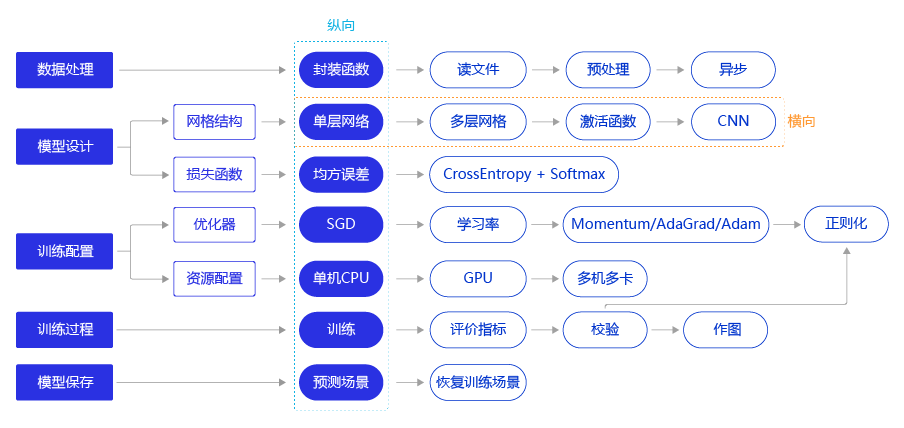
\includegraphics[width=14cm]{figure/深度学习模型实现流程.png}
    \caption{\kaishu 深度学习模型实现流程}\label{Fig: 深度学习模型实现流程}
\end{figure}

\section{数据处理}
% \begin{itemize}
%     \item 
%     \item 
%         \begin{equation*}
%         \mbox{划分数据集}
%         \begin{cases}
%             \mbox{train\_set(训练集):用于确定模型参数。}\\
%             \mbox{val\_set(验证集):用于调节模型超参数(如多个网络结构、正则化权重的最优选择)。}\\
%             \mbox{test\_set(测试集):用于估计应用效果(尽量使用未在模型中应用过的数据)。}
%         \end{cases}
%         \end{equation*}
%         其中训练集必包含训练数据(images)部分和标签(labels 或 ground truthz)部分。

%         验证: validate
%         测试: test 或 evaluate
%     \item 
%         \begin{equation*}
%         \mbox{训练样本集乱序\footnote{通过大量实验发现,模型对最后出现的数据印象更加深刻。训练数据导入后,越接近模型训练结束,最后几个批次数据对模型参数的影响越大。为了避免模型记忆影响训练效果,需要进行样本乱序操作。}}
%         \begin{cases}
%             \mbox{建立顺序编号的ID集合index\_list}\\
%             \mbox{将index\_list乱序}\\
%             \mbox{按乱序后的顺序读取数据}
%         \end{cases}
%         \end{equation*}
%         为什么要乱序?

%         % 实现乱序的操作:
%         % random.shuffle(index\_list)
%     \item 
%         \begin{equation*}
%         \mbox{生成批次数据}
%         \begin{cases}
%             \mbox{设置合理的batch\_size}\\
%             \mbox{将数据shape变为(batch\_size, image\_size)的np.array}\\
%             \mbox{使用python的yield生成器返回数据}
%         \end{cases}
%         \end{equation*}
%     \item 校验数据有效性
% \end{itemize}
    
    \begin{equation*}
    \begin{cases}
    \mbox{读入数据}\\
    \mbox{划分数据集}
        \begin{cases}
            \mbox{train\_set(训练集):用于确定模型参数。}\\
            \mbox{val\_set(验证集):用于调节模型超参数(如多个网络结构、正则化权重的最优选择)。}\\
            \mbox{test\_set(测试集):用于估计应用效果(尽量使用未在模型中应用过的数据)。}
        \end{cases}\\
    \mbox{训练样本集乱序}\footnote{通过大量实验发现,模型对最后出现的数据印象更加深刻。训练数据导入后,越接近模型训练结束,最后几个批次数据对模型参数的影响越大。为了避免模型记忆影响训练效果,需要进行样本乱序操作。}
        \begin{cases}
            \mbox{建立顺序编号的ID集合index\_list}\\
            \mbox{将index\_list乱序}\\
            \mbox{按乱序后的顺序读取数据}
        \end{cases}\\
    \mbox{生成批次数据}
        \begin{cases}
            \mbox{设置合理的batch\_size}\\
            \mbox{将数据shape变为(batch\_size, image\_size)的np.array}\\
            \mbox{使用python的yield生成器返回数据}
        \end{cases}\\
    \mbox{校验数据有效性}
        \begin{cases}
            \mbox{机器校验: assert 图片 与 标签 维度相同}\\
            \mbox{人工校验: print 数据看格式是否符合预期}
        \end{cases}
    \end{cases}
    \end{equation*}

    某基于MNIST数据集的数据生成器的代码实现如下。
    % \begin{lstlisting}[language={Python}]
    \begin{python}
# 定义数据生成器,返回批次数据
def load_data(mode='train'):
    datafile = './work/mnist.json.gz'
    print('loading mnist dataset from {} ......'.format(datafile))
    # 加载json数据文件
    data = json.load(gzip.open(datafile))
    print('mnist dataset load done')
   
    # 读取到的数据区分训练集,验证集,测试集
    train_set, val_set, eval_set = data
    if mode=='train':
        # 获得训练数据集
        imgs, labels = train_set[0], train_set[1]
    elif mode=='valid':
        # 获得验证数据集
        imgs, labels = val_set[0], val_set[1]
    elif mode=='eval':
        # 获得测试数据集
        imgs, labels = eval_set[0], eval_set[1]
    else:
        raise Exception("mode can only be one of ['train', 'valid', 'eval']")
    print("训练数据集数量: ", len(imgs))
    
    # 校验数据
    imgs_length = len(imgs)

    assert len(imgs) == len(labels), \
          "length of train_imgs({}) should be the same as train_labels({})".format(len(imgs), len(labels))
    
    # 获得数据集长度
    imgs_length = len(imgs)
    
    # 定义数据集每个数据的序号,根据序号读取数据
    index_list = list(range(imgs_length))
    # 读入数据时用到的批次大小
    BATCHSIZE = 100
    
    # 定义数据生成器
    def data_generator():
        if mode == 'train':
            # 训练模式下打乱数据
            random.shuffle(index_list)
        imgs_list = []
        labels_list = []
        for i in index_list:
            # 将数据处理成希望的类型
            img = np.array(imgs[i]).astype('float32')
            label = np.array(labels[i]).astype('float32')
            imgs_list.append(img) 
            labels_list.append(label)
            if len(imgs_list) == BATCHSIZE:
                # 获得一个batchsize的数据,并返回
                yield np.array(imgs_list), np.array(labels_list)
                # 清空数据读取列表
                imgs_list = []
                labels_list = []
    
        # 如果剩余数据的数目小于BATCHSIZE,
        # 则剩余数据一起构成一个大小为len(imgs_list)的mini-batch
        if len(imgs_list) > 0:
            yield np.array(imgs_list), np.array(labels_list)
    return data_generator
    \end{python}

    % \end{lstlisting}

\section{模型设计}

    \subsection{多层感知机}
    多层感知器(Multi Layer Perceptron,即 MLP)除了一个输入层和一个输出层以外,包括至少一个隐藏层。多层感知器用来模拟一个非线性函数。


    \subsection{卷积神经网络}

    

\section{训练配置}


    \subsection{反向传播}

    \begin{tikzpicture}
		[L1Node/.style={circle,draw=blue!30,fill=blue!10,very thick, minimum size=10pt},
		L2Node/.style={circle,draw=pink!50,fill=pink!20,very thick, minimum size=10pt}]
		
		% 画输入层结点
		\foreach \x in {1,...,3}  % 循环,使得\x的值依次等于1,2,3
		% \node[结点的样式](结点的名称)at(结点的坐标){结点的内容}
		\node[L1Node] (a_\x) at (0,-1.8*\x){\scriptsize $\alpha^{(1)}_\x$};  
		
		% 画隐藏层结点
		\foreach \x in {1,...,3}
		\node[L2Node] (b_\x) at (1*2.5,-1.8*\x){\scriptsize $\alpha^{(2)}_\x$};
		
		% 画输出层结点
		\foreach \y in {1,2}
		\node[L1Node] (c_\y) at (2*2.5,-1.8*\y-1.8/2){\scriptsize $\alpha^{(3)}_\y$};

        % 添加说明表示
        \node[]at(0*2.5,-0.5){Layer 1};
        \node[]at(1*2.5,-0.5){Layer 2};
        \node[]at(2*2.5,-0.5){Layer 3};

        % 输入特征x
		\foreach \x in {1,2,3}
		\node(x_\x)at(-2,-1.8*\x){$x_\x$};
		
		% 输出数值y
		\node(y_1)at(2*2.5+2,-1.8*1-1.8/2){$y_1$};
		\node(y_2)at(2*2.5+2,-1.8*2-1.8/2){$y_2$};
		
		% 输入特征值与输入层之间的连线
		\foreach \x in {1,2,3} 
		\draw[-stealth](x_\x)--(a_\x);
		
		% 链接输入层到隐藏层之间的连线
		\foreach \x in{1,2,3}
		{\foreach \z in{1,2,3}
			% \draw[线的样式:-{stealth[sep=1pt]}为带箭头的线,[sep箭头距离]
			\draw[-stealth](a_\x)--(b_\z);	
		}
		
		% 链接隐藏层到输出层之间的连线
		\foreach \z in{1,2,3}
		{\foreach \y in{1,2}
			\draw[-stealth](b_\z)--(c_\y);	
		}
		
		% 输出y与输出层之间的连线
		\draw[-stealth](c_1)--(y_1);
		\draw[-stealth](c_2)--(y_2);
		
		% % 添加权值w
		% % \node[结点的样式](结点的名称)at(结点的坐标){结点的内容}
		% \node[](w_1) at (1,-0.65){$w_{41}$};
		% \node[](w_2) at (1,-1.15){$w_{42}$};
		% \node[](w_3) at (1,-1.65){$w_{43}$};
		
		
		% % 隐藏层公式
		% \node[](z) at (2,0.3){$z_j=sigmoid(a_j)$};

		
		% % 输出层公式
		% \node[](y) at (4,-0.5){$y_k=sigmoid(b_k)$};
		

		\node[](w_ji)at(1,-4){$w_{ji}$};
		
	\end{tikzpicture}

    \begin{itemize}
        \item 计算梯度
            \begin{equation}
                \bm{g} \leftarrow \partial_{(\bm{W},b)} \frac{1}{|\mathcal{B}|} \sum_{i\in\mathcal{B}}{L\left(\bm{x}^{(i)},\bm{y}^{(i)},\bm{W},b\right)}
            \end{equation}
        \item 更新参数
            \begin{equation}
                (\bm{W},b) \leftarrow (\bm{W},b) - \eta \bm{g} 
            \end{equation}
    \end{itemize}


    \subsection{特征标准化}

    为了解决输入样本中各个维度的数值差异较大导致 error surface 形状扭曲, 给 gradient descent 带来困难 的问题,引入特征标准化(\emph{Feature Normalization})的方法。

    \begin{itemize}
        \item Batch Normalization
        \item Layer Normalization
        \item lnstance Normalization
        \item Group Normalization
        \item Weight Normalization
        \item Spectrum Normalization
    \end{itemize}

    其中一个常用的标准化方法为 Batch Normalization (BN) 。BN 一次对一个 Batch (记作$\mathcal{B}$,其中第$i$个样本为$N_e\times 1$列向量$\bm{x}^{(i)},\,i=1,\cdots,N_B$) 的输入样本的每一个维度作\emph{standard deviation normalization}:
    \begin{equation}
        % \tilde{\bm{x}}^{(i)}=\frac{\bm{x}^{(i)}-\bm{\mu}}{\bm{\sigma}}
        \tilde{\bm{x}}^{(i)}=\frac{\bm{x}^{(i)}-\mathrm{E}\left[\bm{x}^{(:)}\right]}{\sqrt{\mathrm{Var}\left[\bm{x}^{(:)}\right]}}
    \end{equation}
    % 其中,$\bm{\mu},\bm{\sigma}$分别为一个 Batch 的样本 按对应维度求出的均值和标准差 所组成的向量,其 shape 与 每一个样本的 shape 相同。
    % \begin{subequations}    
    % \begin{equation}
    %     \bm{\mu}=\frac{1}{N_B}\sum_{i=1}^{N_B}{\bm{x}^{(i)}}
    % \end{equation}
    % \begin{equation}
    %     \bm{\sigma}=
    % \end{equation}
    % \end{subequations}
    其中,$\mathrm{E}\left[\bm{x}^{(:)}\right]$ 表示对一个 Batch 内全部样本在同一个维度上求均值,得到一个$N_e\times 1$列向量。求方差$\mathrm{Var}\left[\bm{x}\right]$的过程同理。
        
\section{模型保存}


\section{模型预测}

\chapter{通信原理}

\section{数字频带传输}
        Modulation:用要传输的原始信号$m(t)$控制高频载波信号的某一参量,使它随$m(t)$发生变化。

        这个原始信号$m(t)$称为 \underline{调制信号}或 \underline{基带信号}。
        \begin{itemize}
            \item 模拟调制:$m(t)$为连续时间函数。
            \item 数字调制:调制信号为离散时间序列。
        \end{itemize}

        调制可以根据高频载波信号$C(t)$类型不同分类:
        \begin{itemize}
            \item 正弦波调制:正弦信号作为载波
            \item 脉冲调制:周期性脉冲作为载波
        \end{itemize}

        
        \begin{equation*}
        \mbox{根据调制参量来分类}
        \begin{cases}
            \mbox{正弦波模拟调制}\begin{cases}
                AM\\FM\\PM
            \end{cases}\\
            \mbox{正弦波数字调制}\begin{cases}
                ASK\\FSK\\PSK(相位键控)\\QAM(正交幅度调制)
            \end{cases}\\
            \mbox{脉冲模拟调制}\begin{cases}
                PAM\\PDM\\PPM
            \end{cases}\\
            \mbox{脉冲数字调制}\begin{cases}
                DPAM\\PCM\\DPCM\\ADPCM
            \end{cases}
        \end{cases}
        \end{equation*}


        \subsection{二进制通断键控(On-Off Keying)/二进制幅度键控(2ASK)}
            \begin{itemize}
                \item 传号时有一定幅度,空号时幅度为0。
                \item 可认为相位随机。
                \item 调制信号带宽是基带信号的2倍。
                \item 
            \end{itemize}
        
        \subsection{二进制相移键控(2PSK)}
            2PSK:用二进制数字基带信号控制正弦载波的相位。即码元的载波相位表示数字信息。

            设数字基带信号为双极性非归零信号$s(t)$,则2PSK信号调制过程
            \begin{equation}
                S_\mathrm{2PSK}(t)=s(t)\cos\omega_ct=
                \left\{\begin{aligned}
                    &A\cos(\omega_ct)\quad\mbox{“传号”}\\
                    -&A\cos(\omega_ct)\quad\mbox{“空号”}
                \end{aligned}\right.
                \qquad 0\leqslant t\leqslant T_b
            \end{equation}
            
        \begin{figure}[htp]
            \begin{center}
                \begin{tikzpicture}
                    [
                    node distance=6mm,
                    point/.style={circle,inner sep=0pt,minimum size=2pt,fill=black},
                    rect1/.style={shape = rectangle, draw ,text width = 1.2cm, align = flush center, minimum height = 1.2cm, inner sep=2mm},
                    ]
                    % % 辅助网格 标注原点
                    % \draw[step=1,help lines] (-5,-3) grid (5,3);
                    % \node [point] at (0,0) {};
                    % %
                    \node[label=below:{$S_\mathrm{2PSK}(t)$}] (in) {输入};
                    \node[rect1, right=of in] (信道) {信道};
                    \node[rect1, xshift=10mm, right=of 信道] (BPF) {BPF};
                    \node[draw, xshift=5mm, thick, circle, inner sep=-1pt, right=of BPF] (MUL) {\fontsize{20.74}{18}$\displaystyle \times$};
                    \node[rect1, right=of MUL] (LPF) {LPF};
                    \node[rect1, xshift=5mm, right=of LPF] (抽样判决器) {抽样\\判决器};
                    \node[xshift=5mm, label=below:{$P_e$}, right=of 抽样判决器] (out) {输出};

                    \node[below=of 信道] (噪声) {$n_i(t)$};
                    \node[below=of MUL, yshift=-4mm] (本振) {本地载波};
                    \node[below=of 抽样判决器] (定时脉冲) {定时脉冲};
                    %
                    \path[->,>=latex]
                        (in) edge node[] {} (信道)
                        (信道) edge node[below, pos=0.3] {$y_i(t)$} (BPF)
                        (BPF) edge node[below] {$y(t)$} (MUL)
                        (MUL) edge node[] {} (LPF)
                        (LPF) edge node[below] {$x(t)$} (抽样判决器)
                        (抽样判决器) edge node[] {} (out)

                        (噪声) edge (信道)
                        (本振) edge node [right, pos=0.4] {$2\cos\omega_c t$} (MUL)
                        (定时脉冲) edge (抽样判决器)
                    ;
                    \node [draw=black!50, dashed, very thick, rectangle, inner xsep = 4.7cm, inner ysep = 1.6cm, yshift=-0.4cm, xshift=1cm] at (MUL) {};
                \end{tikzpicture}
            \end{center}
            \caption{\kaishu 2PSK相干解调系统}\label{Fig: 2PSK相干解调系统}
        \end{figure}

        经过BPF,加性高斯白噪声变为窄带高斯噪声,有效信号的部分不变:
        \begin{equation}
            y(t)=
            \left\{\begin{aligned}{}
                [ &k_BA+n_c(t)]\cos\omega_ct-n_s(t)\sin\omega_ct\;,\; \mbox{"1"}\\
                [-&k_BA+n_c(t)]\cos\omega_ct-n_s(t)\sin\omega_ct\;,\; \mbox{"0"}
            \end{aligned}\right.
            \quad 0\leqslant t\leqslant T_b
        \end{equation}
        
        本振信号与BPF输出相乘(注意本振信号相位可能未对准),并经过LPF:
        \begin{equation}
            \begin{aligned}
                x(t)&=\mathrm{LPF}\left\{2[\pm k_BA+n_c(t)]\cos(\omega_ct)\cos(\omega_ct+\Delta\theta)-2n_s(t)\sin(\omega_ct)\cos(\omega_ct+\Delta\theta)\right\}\\
                &=\mathrm{LPF}\{2[\pm k_BA+n_c(t)][\cos^2(\omega_ct)\cos \Delta \theta-\cos(\omega_ct)\sin(\omega_ct)\sin \Delta \theta]\\
                                & \qquad \qquad -2n_s(t)[-\sin^2(\omega_ct)\sin \Delta \theta+\sin(\omega_ct)\cos\omega_ct\cos \Delta \theta]\}\\
                &=k_L[\pm k_BA+n_c(t)]\cos \Delta \theta +k_Ln_s(t)\sin \Delta \theta\\
            \end{aligned}
        \end{equation}
        
        理想情况下$\Delta \theta=0$,
        \begin{equation}
            x(t)=
            \left\{\begin{aligned}{}
                k_L [&k_BA+n_c(t)]\;,\quad \mbox{"1"}\\
                k_L[-&k_BA+n_c(t)]\;,\quad \mbox{"0"}
            \end{aligned}\right.
            \qquad 0\leqslant t\leqslant T_b
        \end{equation}
        
        最恶劣情况下$\Delta \theta=\pi$,
        \begin{equation}
            x(t)=
            \left\{\begin{aligned}{}
                k_L [-&k_BA-n_c(t)]\;,\quad \mbox{"1"}\\
                k_L[&k_BA-n_c(t)]\;,\quad \mbox{"0"}
            \end{aligned}\right.
            \qquad 0\leqslant t\leqslant T_b
        \end{equation}
        对于2PSK信号,这种情况导致解调系统反相工作。因此本地载波相位会导致输出绝对码反相,这种现象称为相位模糊。

        \subsection{二进制差分相移键控(2DPSK)}
        为解决2PSK信号存在的相位模糊问题,引入2DPSK。

        设数字基带信号为双极性非归零信号$s(t)$,对应的绝对码记作$\left\{a_n\right\}$,经过差分编码得到相对码$\left\{b_n\right\}$:
        \begin{equation}
            b_n=a_n\oplus b_{n-1}
        \end{equation}
        其中$\oplus$表示模二加,这里等价为异或运算。$\left\{b_n\right\}$的初始参考设为$0$。

        二进制下,相对码的“0”和“1”分别表示
        \begin{equation}
            b_n=
            \left\{\begin{aligned}
                &0\;,\quad \varphi_n-\varphi_{n-1}=0\\
                &1\;,\quad \varphi_n-\varphi_{n-1}=\pm \pi
            \end{aligned}\right.
        \end{equation}

        反过来由相对码得出绝对码的过程称为差分译码:
        \begin{equation}
            a_n=b_n\oplus b_{n-1}
        \end{equation}

        \begin{figure}[htp]
            \begin{center}
                \begin{tikzpicture}[scale=1.5,
                    point/.style={circle,inner sep=0pt,minimum size=2pt,fill=black},]
                    % % 辅助网格 标注原点
                    % \draw[step=1,help lines] (-4,-2) grid (4,2);
                    % \node [point] at (0,0) {};
                    %
                    \coordinate (s) at (-3,0);
                    \coordinate (z) at (2,0);


                    % 差分编码
                    \draw (s)++(-2,0) node (A) {$a_n$};
                    \draw (s)++(-1,0) node[inner sep=-1pt] (S){\fontsize{20.74}{18}$\oplus$};
                    \draw (s)++(0,-1) node[draw] (D) {$T_B$};
                    \draw (s)++(1,0) node (B) {$b_n$};
                    %
                    \path[->,>=latex]
                        (A) edge (S)
                        (S) edge (B)
                        (s) edge (D)
                    ;
                    \node [point] at (s) {};
                    \draw (s)++(-1,-1) -- (D.west)
                        (s)++(-1,-1) edge[->,>=latex] node[left] {$b_{n-1}$} (S.south) ;
                    % 差分译码
                    \draw (z)++(-2,0) node (A) {$b_n$};
                    \draw (z)++(-1,-1) node[draw] (D) {$T_B$};
                    \draw (z)++(0,0) node[inner sep=-1pt] (S){\fontsize{20.74}{18}$\oplus$};
                    \draw (z)++(1,0) node (B) {$a_n$};
                    %
                    \path[->,>=latex]
                        (A) edge (S)
                        (S) edge (B)
                        (z)++(-1,0) edge (D)
                    ;
                    \draw (z)++(-1,0) node[point]  {};
                    \draw (z)++(0,-1) -- (D.east)
                        (z)++(0,-1) edge[->,>=latex] node[right] {$b_{n-1}$} (S.south) ;

                \end{tikzpicture}
            \end{center}
            \caption{\kaishu 差分译码和差分解码}\label{Fig: 差分译码和差分解码}
        \end{figure}

        绝对码$\left\{a_n\right\}$的2DPSK信号,就是相对码$\left\{b_n\right\}$的2PSK信号。即经过差分译码后,可通过产生PSK信号的方式产生DPSK信号。

        2DPSK信号的解调可以使用相干解调加差分译码的方式,也可以用差分相干解调法
        \begin{figure}[htp]
            \begin{center}\resizebox{\textwidth}{!}{
                \begin{tikzpicture}
                    [
                    node distance=6mm,
                    point/.style={circle,inner sep=0pt,minimum size=2pt,fill=black},
                    rect1/.style={shape = rectangle, draw ,text width = 1.2cm, align = flush center, minimum height = 1.2cm, inner sep=2mm},
                    ]
                    % % 辅助网格 标注原点
                    % \draw[step=1,help lines] (-5,-3) grid (5,3);
                    % \node [point] at (0,0) {};
                    % %
                    \node[label=below:{$S_\mathrm{2DPSK}(t)$}] (in) {输入};
                    \node[rect1, right=of in] (信道) {信道};
                    \node[rect1, xshift=10mm, right=of 信道] (BPF) {BPF};
                    \node[draw, xshift=5mm, thick, circle, inner sep=-1pt, right=of BPF] (MUL) {\fontsize{20.74}{18}$\displaystyle \times$};
                    \node[rect1, right=of MUL] (LPF) {LPF};
                    \node[rect1, xshift=5mm, right=of LPF] (抽样判决器) {抽样\\判决器};
                    \node[rect1, xshift=7mm, right=of 抽样判决器] (差分译码) {差分\\译码};
                    \node[xshift=5mm, label=below:{$a_n$}, right=of 差分译码] (out) {输出};

                    \node[below=of 信道] (噪声) {$n_i(t)$};
                    \node[below=of MUL, yshift=-4mm] (本振) {本地载波};
                    \node[below=of 抽样判决器] (定时脉冲) {定时脉冲};
                    %
                    \path[->,>=latex]
                        (in) edge node[] {} (信道)
                        (信道) edge node[below, pos=0.3] {$y_i(t)$} (BPF)
                        (BPF) edge node[below] {$y(t)$} (MUL)
                        (MUL) edge node[] {} (LPF)
                        (LPF) edge node[below] {$x(t)$} (抽样判决器)
                        (抽样判决器) edge node[below, pos=0.7] {$b_n$} (差分译码)
                        (差分译码) edge node[] {} (out)

                        (噪声) edge (信道)
                        (本振) edge node [right, pos=0.4] {$2\cos\omega_c t$} (MUL)
                        (定时脉冲) edge (抽样判决器)
                    ;
                    \node [draw=black!50, dashed, very thick, rectangle, inner xsep = 4.7cm, inner ysep = 1.6cm, yshift=-0.4cm, xshift=1cm] at (MUL) {};
                \end{tikzpicture}}
            \end{center}
            \caption{\kaishu 2DPSK相干解调系统}\label{Fig: 2DPSK相干解调系统}
        \end{figure}

        相干解调部分和PSK解调相同,若只考虑一个码元内的波形:

    \section{移动通讯}
    \subsection{5G}

    \subsection{6G}

    覆盖率(到90\%)、传输速度(Tbps)、低延时(1ms)、定位精度、可靠性、低功耗、智能水平。

    
    

\chapter{电子电路}

\section{电源}

    \subsection{同步Buck}
    开关频率为$f_s$,则周期$T_s=\frac{1}{f_s}$,MTOP(同步Buck,上管称开关管,记MTOP,下管称续流管,记MBOT)导通时长为
    \begin{equation}
        T_\mathrm{on}=D\cdot\frac{1}{f_s}
    \end{equation}
    $D$为占空比。
    电感开始储能,流过的电流增大,电感上电压左正($V_\mathrm{in}$)右负($V_\mathrm{out}$),伏秒积:
    \begin{equation}
        (V_\mathrm{in}-V_\mathrm{out})DT_s
    \end{equation}
    (伏秒积反映了电感中电流的增量。这是因为电感特性:电感电压等于感量乘以电流的时间变化率。)
    其本质为流过的电流变化:
    \begin{equation}
        i_L(t)=i_L(0)+\frac{V_\mathrm{in}-V_\mathrm{out}}{L}t
    \end{equation}
    因此电流增量:
    \begin{equation}
        \Delta I_L=i_L(T_\mathrm{on})-i_L(0)=\frac{\left(V_\mathrm{in}-V_\mathrm{out}\right)D}{Lf_s}
    \end{equation}
    MTOP关断,MBOT导通时长为:
    \begin{equation}
        T_\mathrm{off}=(1-D)\cdot\frac{1}{f_s}
    \end{equation}
    电感向外输出电能,流过的电流逐渐减小,电感上电压左负(0)右正($V_\mathrm{out}$),伏秒积:
    \begin{equation}
        V_\mathrm{out}(1-D)T_s
    \end{equation}
    在稳态下,电感上的电流纹波$\Delta I$,应该等于MTOP开通期间输出电流的增加量,也等于其关断期间输出电流的减小量。
    所以开通和关断期间电感的伏秒积相等,
    \begin{equation}
        (V_\mathrm{in}-V_\mathrm{out})DT_s=V_\mathrm{out}(1-D)T_s
    \end{equation}
    可得:
    \begin{equation}
        D=\frac{V_\mathrm{out}}{V_\mathrm{in}}
    \end{equation}
    因此输出电流纹波:
    \begin{equation}
        \Delta I_L=\frac{\left(V_\mathrm{in}-V_\mathrm{out}\right)D}{Lf_s}=\frac{V_\mathrm{out}\left(1-\frac{V_\mathrm{out}}{V_\mathrm{in}}\right)}{Lf_s}
    \end{equation}
    \fbox{\makecell[{{p{16cm}}}]{由于输出电压的需求是确知的,开关频率由IC确定(为绕开汽车FM频段,一般固定在\SI{500}{\kilo\hertz}数量级或者大于2\si{\mega\hertz}),我们可以利用的结论通常总结为:输入电压越高,纹波越大;电感越大,纹波越小。}}

    有了电流纹波,就可以据此计算电感参数。一般原则是电流纹波为输出电流$I_\mathrm{out}$的$20\% \sim 40\%$。取小主要受到空间成本、动态响应等方面的约束,取大主要受到电容耐受、负载端PSRR指标的约束。


    个人观点:在负载为较高精度的模拟电路下,尽量选大电感加大耐压的电容,并做好负载IC的瞬态抑制和浪涌保护。


    电感值选取:
    \begin{equation}
        L=\frac{V_\mathrm{out}\left(1-\frac{V_\mathrm{out}}{V_\mathrm{in,max}}\right)}{\Delta I f_s}
    \end{equation}
    取输入电压最大值就是为了考虑最坏情况——如果$\Delta I$最大,电路能满足要求,那么其他情况纹波只会更小,更能满足要求。


    电感选取还要注意饱和电流的问题:铁氧体电感存在硬饱和、磁漏、体积大的问题,当电流超过一定值后电感感量急剧下降;一体成型的粉芯电感软饱和,但可能存在感值小、散热慢等问题。
    通常取
    \begin{equation}
        I_{L(max)}=I_\mathrm{out}+0.5 \Delta I
    \end{equation}
    作为对电感饱和电流参数的标准。必须选择饱和电流比该值大的电感。
    \begin{center}
        (饱和电流常定义为使L下降额定值的30\%处的电流)
    \end{center}


    通过电流纹波计算电压纹波:
    \begin{equation}
        V_\mathrm{ripple}=\Delta I\left(\frac{1}{8f_sC_\mathrm{out}}+(ESR)_{C_\mathrm{out}}\right)
    \end{equation}
    输出电压纹波有容性分量和阻性分量,分别由输出滤波电容的容值(不足)和其ESR(过大)引起。

    \subsection{PFC}
    功率因数校正(Power Factor Correction, PFC)电路,用于防止用电器产生的杂波影响到电网。
    
    LG=logic ground 逻辑地,也是数字地
    
    
    PE=power earth是电源地

    FG是保护地,外壳接地


\end{document}
